\chapter*{Введение}
\addcontentsline{toc}{chapter}{Введение}

Топологический анализ данных -- это новая область анализа данных, которая своими корнями уходит в алгебраическую топологию. Она возникла в результате прорывных работ Герберта Эдельсбруннера \cite{Edelsbrunner et al} и Гуннара Карлссона \cite{Carlsson and Zomorodian} по устойчивым гомологиям, которые впоследствии стали основными инструментами данной сферы. 

В задачах анализа данных большое значение имеет информация о геометрической и топологической структуре исследуемых данных. Зачастую такая структура позволяет выявить некоторые закономерности между различными переменными. Помимо этого, существует также гипотеза о многообразии, которая утверждает, что реальные данные, представленные облаком точек из $\mathbb{R}^n$ лежат на некотором $d$-многообразии, где $d \leq n$. 

Так, в последнее время, появляется все больше работ, которые направлены на изучение т.н. латентного пространства некоторых видов нейросетей: VAE и GAN. Эти нейросети в ходе обучения пытаются воссоздать то самое многомерное многообразие, на котором лежат данные, например, изображения. Латентное пространство зачастую скрыто во многих методах анализа данных, и содержит всю необходимую информацию, поэтому изучение его свойств крайне важно. Топологический анализ данных, в силу своего топологического фундамента, может быть крайне полезен для такой задачи. Данная тема является популярной темой современных исследований в этой области.

%[тут должны быть ссылки на работы по топ автокодировщикам, латент пр-ву ганов и вае, по персист гомол латент спейса]


Данная работа посвящена обзору современных инструментов топологического анализа данных, а также применению персистентных гомологий, которые являются основным инструментом данного подхода, к задаче классификации на примере стандартного для классификации датасета MNIST.  

Задача классификации -- это задача машинного обучения и анализа данных, в которой есть конечное множество {\it объектов}, разделенных на конечное число {\it классов}, т.е. на конечное число попарно не пересекающихся множеств, наделенных некоторым свойством. Такое заданное множество называется {\it выборкой}. Целью данной задачи является построение алгоритма, который, на основе имеющейся информации в выборке, будет способен определить, к какому классу относится новый объект, т.е. объект, не находящийся в исходной выборке.

Таким образом в данной работе будет применен аппарат персистентных гомологий для задачи классификации изображений датасета MNIST. Датасет MNIST -- это датасет, который состоит из 60000 изображений для обучения, а также 10000 изображений для тестирования, где каждое изображение является черно-белым изображением рукописной цифры от $0$ до $9$. Типичное изображение из данного датасета представлено на рис. \ref{mnist-example}. Данный датасет считается одним из стандартных датасетов для обучения различных методов распознавания изображений с помощью машинного обучения, причем в первую очередь для методов, основанных на нейронных сетях. Однако, в следствие нейросетевого бума, который случился в последнее десятилетие, а в частности с появлением и развитием сверточных нейронных сетей, данный датасет слегка утратил свою актуальность -- современные нейросети выдают почти 100-процентную точность, и для обучения нейросетей сейчас используют другие датасеты. 

\begin{figure}[!htbp]
	\begin{center}
		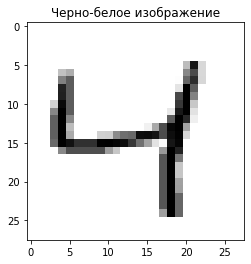
\includegraphics[width=0.5\textwidth]{grayscaleImage.png}\\
		\caption{Пример изображения из датасета MNIST}
		\label{mnist-example}
	\end{center}
\end{figure}

Однако при поиске новых подходов к классификации изображений все еще используют датасет MNIST. Поэтому в данной работе будет решена задачи классификации изображений именно с использованием данного датасета: топологический анализ данных, и в частности устойчивые гомологии -- это новые инструменты для решения задачи классификации, в этой области все больше выходят современных исследований.
